\vspace{-0.2cm}
\subsection{Experimental Evaluation of COMBO}
\label{sec:combo_exp}
\vspace{-0.2cm}

In our experiments, we aim to answer the follow questions: \textbf{(1)} Can COMBO generalize better than previous offline model-free and model-based approaches in a setting that requires generalization to tasks that are different from what the behavior policy solves? \textbf{(2)} How does COMBO compare with prior work in tasks with high-dimensional image observations?, \textbf{(3)} How does COMBO compare to prior offline model-free and model-based methods in standard offline RL benchmarks?

To answer those questions, we compare COMBO to several prior methods. In the domains with compact state spaces, we compare with recent model-free algorithms like BEAR~\citep{kumar2019stabilizing}, BRAC~\citep{wu2019behavior}, and the CQL~\citep{kumar2020conservative} algorithm presented in the previous section; as well as MOPO~\citep{yu2020mopo} {and MOReL~\citep{kidambi2020morel} which are two recent model-based algorithms}. In addition, we also compare with an offline version of SAC~\citep{haarnoja2018soft} (denoted as SAC-off), and behavioral cloning (BC). In high-dimensional image-based domains, which we use to answer question (3), we compare to LOMPO~\citep{Rafailov2020LOMPO}, which is a latent space offline model-based RL method that handles image inputs, latent space MBPO (denoted LMBPO), similar to \citet{janner2019trust} which uses the model to generate additional synthetic data, the fully offline version of SLAC \citep{lee2019SLAC} (denoted SLAC-off), which only uses a variational model for state representation purposes, and CQL from image inputs. To our knowledge, CQL, MOPO, and LOMPO are representative of state-of-the-art model-free and model-based offline RL methods. Hence we choose them as comparisons to COMBO. For more details of our experimental set-up, comparisons, and hyperparameters, see Appendix~\ref{app:details}.

\vspace{-0.1cm}
\subsubsection{Results on tasks that require generalization}
\label{sec:generalization_exps}
\vspace{-0.2cm}

\begin{table}
\centering
\scriptsize
\resizebox{0.99\textwidth}{!}{\begin{tabular}{l|r|r|r|r|r|r}
\toprule 
\textbf{Environment} & \stackanchor{\textbf{Batch}}{\textbf{Mean}} & \stackanchor{\textbf{Batch}}{\textbf{Max}} & \stackanchor{\textbf{COMBO}} {\textbf{(Ours)}} & \textbf{MOPO} & {\textbf{MOReL}} & \textbf{CQL}\\ \midrule
halfcheetah-jump & -1022.6 & 1808.6 & \textbf{5392.7} & 4016.6 & {3228.7} & 741.1\\
ant-angle & 866.7 & 2311.9 & \textbf{2764.8} & 2530.9 & {2660.3} & 2473.4\\
sawyer-door-close & 5\% & 100\% & \textbf{100}\% & 65.8\% & 42.9\% & 36.7\%\\
\bottomrule
\end{tabular}}
\vspace{-0.2cm}
\caption{
\footnotesize Average returns of \texttt{halfcheetah-jump} and \texttt{ant-angle} and average success rate of \texttt{sawyer-door-close} that require out-of-distribution generalization. All results are averaged over 3 random seeds. We include the mean and max undiscounted return / success rate of the episodes in the batch data (under Batch Mean and Batch Max, respectively) for comparison.
}
\vspace{-0.3cm}
\label{tbl:generalize}
\normalsize
\end{table}

To answer question (1), we use the two environments \texttt{halfcheetah-jump} and \texttt{ant-angle} constructed in \citet{yu2020mopo}, which requires the agent to solve a task that is different from what the behavior policy solved. In both environments, the offline dataset is collected by policies trained with the original reward functions of \texttt{halfcheetah} and \texttt{ant}, which reward the halfcheetah and the ant to run as fast as possible. The behavior policies are trained with SAC with 1M steps and we take the full replay buffer as the offline dataset. Following \citet{yu2020mopo}, we relabel the rewards in the offline datasets to reward the halfcheetah to jump as high as possible and the ant to run to the top corner with a 30 degree angle as fast as possible. Following the same manner, we construct a third task \texttt{sawyer-door-close} based on the environment in \citet{yu2020meta, Rafailov2020LOMPO}. In this task, we collect the offline data with SAC policies trained with a sparse reward function that only gives a reward of 1 when the door is \textit{opened} by the sawyer robot and 0 otherwise. The offline dataset is similar to the ``medium-expert`` dataset in the D4RL benchmark since we mix equal amounts of data collected by a fully-trained SAC policy and a partially-trained SAC policy. We relabel the reward such that it is 1 when the door is \textit{closed} and 0 otherwise. Therefore, in these datasets, the offline RL methods must generalize beyond behaviors in the offline data in order to learn the intended behaviors. We visualize \texttt{sawyer-door-close} on the right in Figure~\ref{fig:visual} in Appendix~\ref{app:image_details}.

We present the results on the three tasks in Table~\ref{tbl:generalize}. {COMBO significantly outperforms MOPO, MOReL and CQL, two representative model-based methods and one representative model-free methods respectively}, in the \texttt{halfcheetah-jump} and \texttt{sawyer-door-close} tasks, and {achieves an approximately 8\%, 4\% and 12\% improvement over MOPO, MOReL and CQL respectively on the \texttt{ant-angle} task}. {These results validate that COMBO achieves better generalization results in practice by behaving less conservatively than prior model-free offline methods (compare to CQL, which doesn't improve much) and more robustly than prior model-based offline methods (compare to MOReL and MOPO).}

% \subsubsection{Empirical analysis on uncertainty estimation in offline model-based RL}
% \label{sec:uq}

% \begin{figure}
%     \vspace{-0.5cm}
%         \centering
%         % 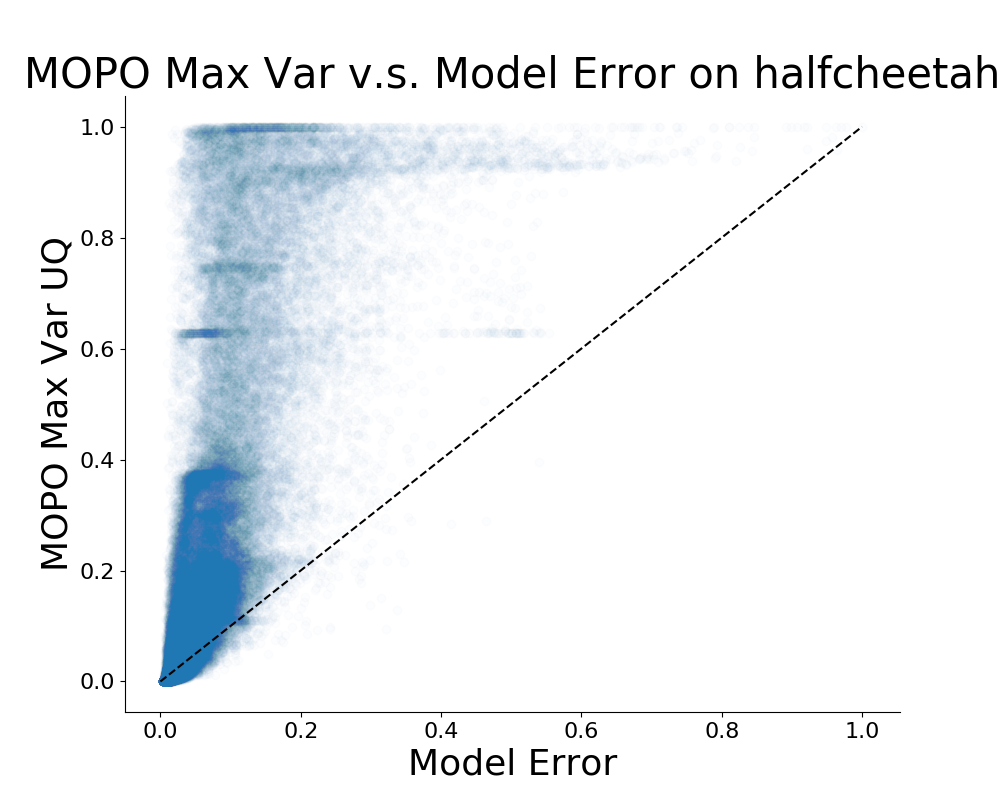
\includegraphics[width=0.47\linewidth]{halfcheetah_medium_corr_var_ood.png}
%         % 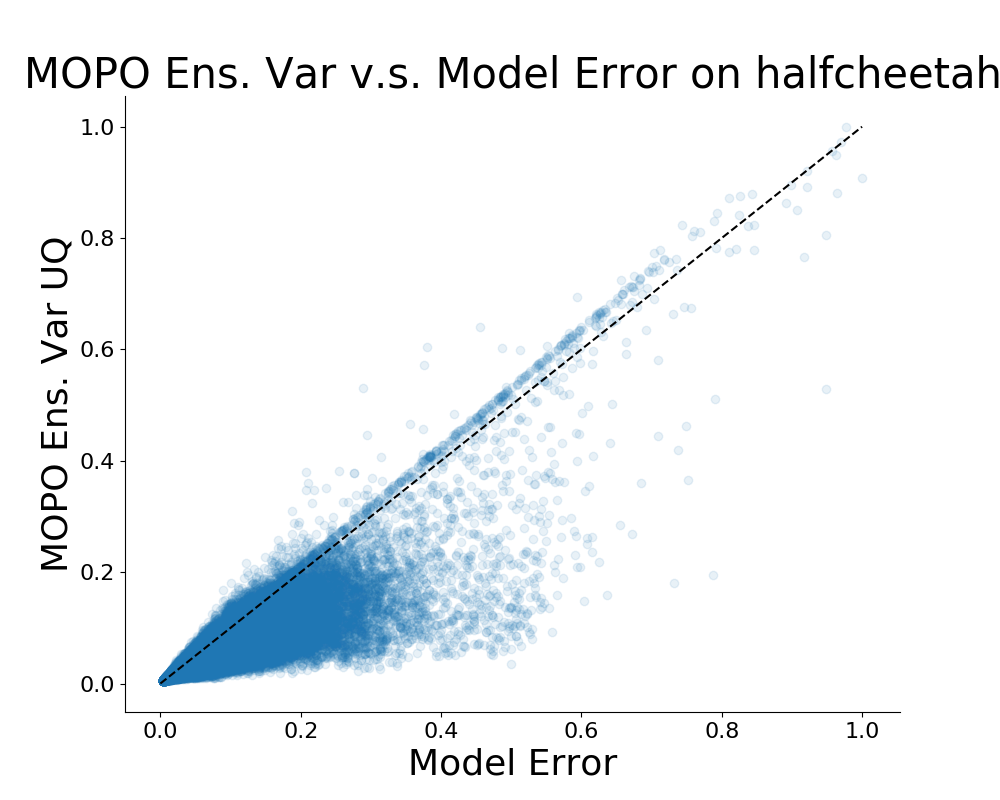
\includegraphics[width=0.47\linewidth]{halfcheetah_medium_corr_lip_ens_ood.png}
%         % 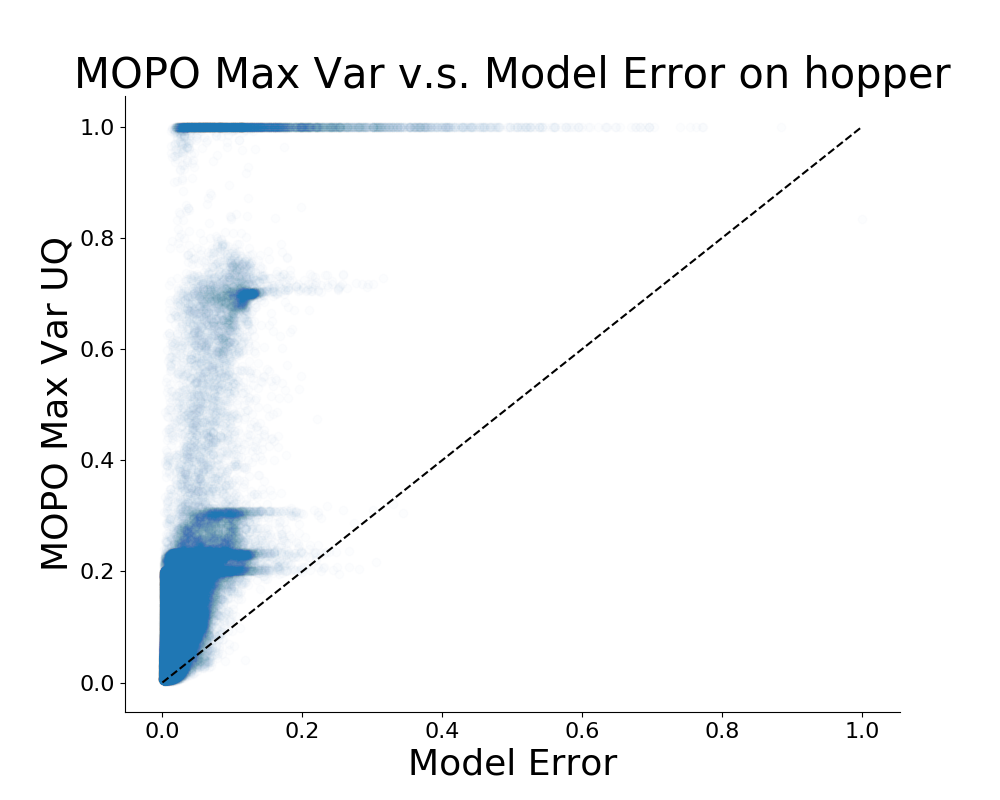
\includegraphics[width=0.47\linewidth]{hopper_medium_corr_var_ood.png}
%         % 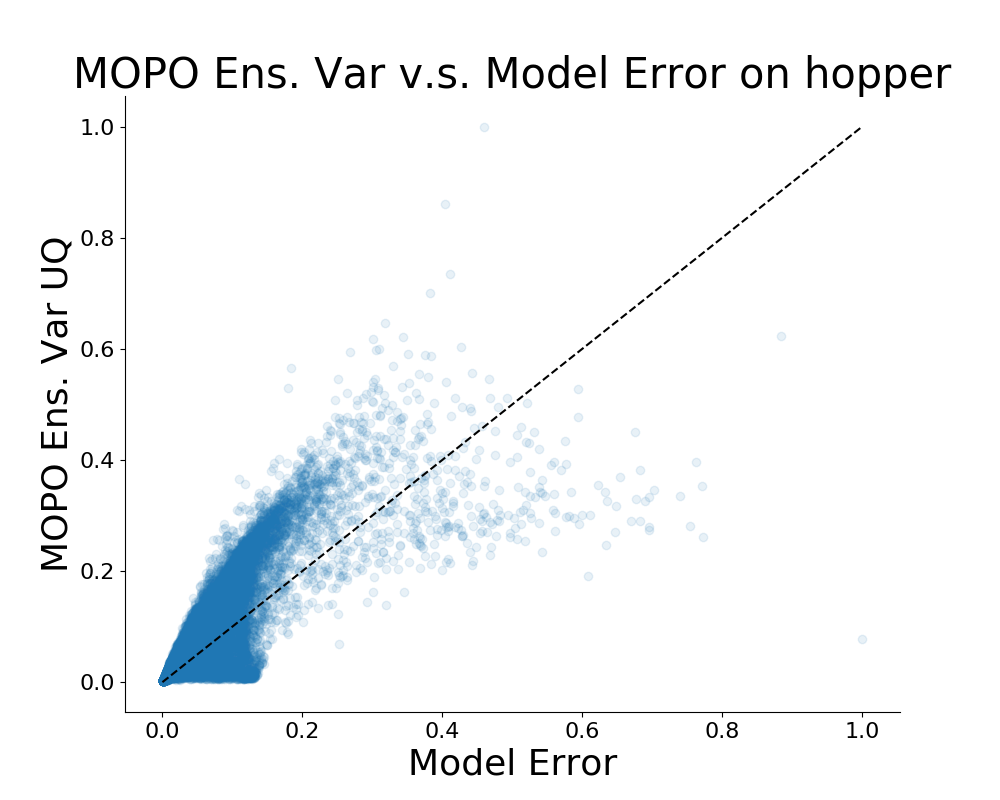
\includegraphics[width=0.47\linewidth]{hopper_medium_corr_lip_ens_ood.png}
%         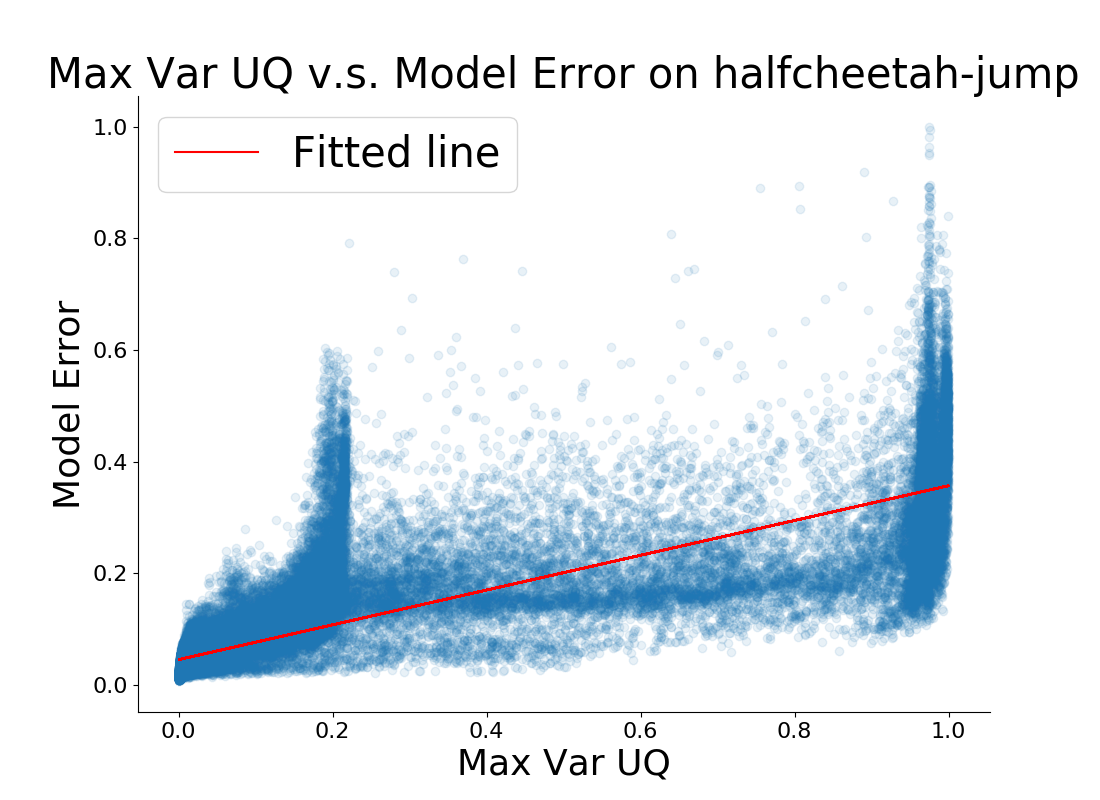
\includegraphics[width=0.45\textwidth]{chapters/combo/halfcheetah_jump_linear_regression_lip_ens_ood.png}
%         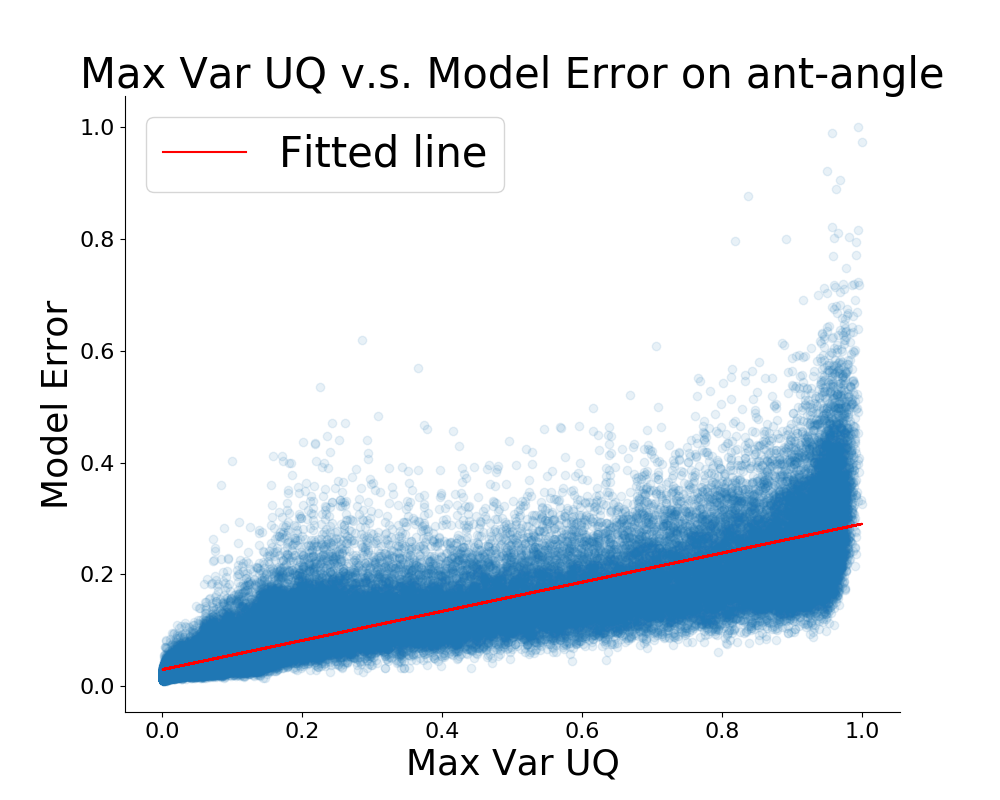
\includegraphics[width=0.41\textwidth]{chapters/combo/ant_angle_linear_regression_lip_ens_ood.png}
%         \vspace{-0.2cm}
%         \caption{\footnotesize {We visualize the fitted linear regression line between the model error and two uncertainty quantification methods maximum learned variance over the ensemble (denoted as \textbf{Max Var}) on two tasks that test the generalization abilities of offline RL algorithms (\texttt{halfcheetah-jump} and \texttt{ant-angle}). We show that \textbf{Max Var} struggles to predict the true model error. Such visualizations indicates that uncertainty quantification is challenging with deep neural networks and could lead to poor performance in model-based offline RL in settings where out-of-distribution generalization is needed. In the meantime, COMBO addresses this issue by removing the burden of performing uncertainty quantification.}}
%         \label{fig:uq}
%         \vspace{-0.4cm}
% \end{figure}

% {To further understand why COMBO outperforms prior model-based methods in tasks that require generalization, we argue that one of the main reasons could be that uncertainty estimation is hard in these tasks where the agent is required to go further away from the data distribution. To test this intuition, we perform empirical evaluations to study whether uncertainty quantification with deep neural networks, especially in the setting of dynamics model learning, is challenging and could cause problems with uncertainty-based model-based offline RL methods such as MOReL~\citep{kidambi2020morel} and MOPO~\citep{yu2020mopo}. In our evaluations, we consider maximum learned variance over the ensemble (denoted as \textbf{Max Var}) $\max_{i=1,\dots,N}\|\Sigma^i_\theta(\bs, \mathbf{a})\|_\text{F}$ (used in MOPO).

% We consider two tasks \texttt{halfcheetah-jump} and \texttt{ant-angle}. We normalize both the model error and the uncertainty estimates to be within scale $[0, 1]$ and performs linear regression that learns the mapping between the uncertainty estimates and the true model error. As shown in Figure~\ref{fig:uq}, on both tasks, \textbf{Max Var} is unable to accurately predict the true model error, suggesting that uncertainty estimation used by offline model-based methods is not accurate and might be the major factor that results in its poor performance. Meanwhile, COMBO circumvents challenging uncertainty quantification problem and achieves better performances on those tasks, indicating the effectiveness of the method.}

\vspace{-0.2cm}
\subsubsection{Results on Image-Based Tasks}
\vspace{-0.2cm}
To answer question (2), we evaluate COMBO on two image-based tasks: the standard walker (\texttt{walker-walk}) task from the the DM Control suite \cite{tassa2018deepmind} and a visual door opening environment with a Sawyer robotic arm (\texttt{sawyer-door}) as used in Section~\ref{sec:generalization_exps}. For the walker task we construct 4 datasets: medium-replay (M-R), medium (M), medium-expert (M-E), and expert, similar to \citet{fu2020d4rl}, each consisting of 200 trajectories. For \texttt{sawyer-door} task we use only the medium-expert and the expert datasets, due to the sparse reward -- the agent is rewarded only when it successfully opens the door. Both environments are visulized in Figure~\ref{fig:visual} in Appendix~\ref{app:image_details}. To extend COMBO to the image-based setting, we follow \citet{Rafailov2020LOMPO} and train a recurrent variational model using the offline data and use train COMBO in the latent space of this model.

\begin{table}
\vspace{-0.2cm}
\centering
\scriptsize
\resizebox{0.75\textwidth}{!}{\begin{tabular}{l|l|r|r|r|r|r}
\toprule
\textbf{\!\!\!Dataset\!\!} & \textbf{Environment} & \vtop{\hbox{\bf \strut COMBO (Ours)}}  & \textbf{LOMPO}& \textbf{LMBPO}& \vtop{\hbox{\bf \strut SLAC-Off}} & \textbf{CQL}\\ \midrule
\!\!\!M-R           & walker\_walk & \textbf{69.2}  & 66.9 & 59.8  & 45.1 & 15.6          \\
\!\!\!M             & walker\_walk & 57.7  & 60.2 & \textbf{61.7}  & 41.5 & 38.9          \\
\!\!\!M-E           & walker\_walk & 76.4  & \textbf{78.9} & 47.3  & 34.9 & 36.3          \\
\!\!\!expert        & walker\_walk & \textbf{61.1}  & 55.6 & 13.2  & 12.6 & 43.3          \\
\!\!\!M-E\!\!\!     & sawyer-door &\textbf{100.0\%} & \textbf{100.0\%}& 0.0\%  & 0.0\% & 0.0\% \\
\!\!\!expert\!\!\!        & sawyer-door &\textbf{96.7\%}  & 0.0\%           & 0.0\% & 0.0\%  & 0.0\% \\
\bottomrule
\end{tabular}}
\vspace{-0.2cm}
\caption{\footnotesize Results for vision experiments. %
For the Walker task each number is the normalized score proposed in \cite{fu2020d4rl} of the policy at the last iteration of training, averaged over 3 random seeds. For the Sawyer task, we report success rates over the last 100 evaluation runs of training. For the dataset, M refers to medium, M-R refers to medium-replay, and M-E refers to medium expert.}
\label{tbl:vision}
\normalsize
\vspace{-0.5cm}
\end{table}

We present results in Table~\ref{tbl:vision}. On the \texttt{walker-walk} task, COMBO performs in line with LOMPO and previous methods. On the more challenging Sawyer task, COMBO matches LOMPO and achieves 100\% success rate on the medium-expert dataset, and substantially outperforms all other methods on the narrow expert dataset, achieving an average success rate of 96.7\%, when all other model-based and model-free methods fail. 
%%CF: Need to describe the walker results
%%RR: Added a sentence, perhaps shouldn't focus on it too much - pefromance is comparable to LOMPO?


\vspace{-0.2cm}
\subsubsection{Results on the D4RL Tasks}
\label{sec:d4rl_exps}
\vspace{-0.2cm}

{Finally, to answer the question (3)}, we evaluate COMBO on the OpenAI Gym~\citep{brockman2016openai} domains in the D4RL benchmark~\citep{fu2020d4rl}\footnote{Note that these results are on the older ``v0'' versions of the D4RL tasks, which are different from ``v2'' versions. Methods attain significantly different performance numbers on v2 compared to v0.}, which contains three environments (halfcheetah, hopper, and walker2d) and four dataset types (random, medium, medium-replay, and medium-expert). We include the results in Table~\ref{tbl:d4rl}. The numbers of BC, SAC-off, BEAR, BRAC-P and BRAC-v are taken from the D4RL paper, while the results for MOPO, {MOReL} and CQL are based on their respective papers~\citep{yu2020mopo,kumar2020conservative}. 
{COMBO achieves the best performance in 9 out of 12 settings and comparable result in 1 out of the remaining 3 settings (hopper medium-replay).}
% COMBO achieves the best performance in 9 out of 12 settings while attaining similar performance to the best-performing method in the remaining 3 settings. 
As noted by \citet{yu2020mopo} and \citet{Rafailov2020LOMPO}, model-based offline methods are generally more performant on datasets that are collected by a wide range of policies and have diverse state-action distributions (random, medium-replay datasets)
%%CF: This disputes the results because CQL does better on medium-expert than MOPO.
%%TY.2.3: I moved medium-expert to datasets with narrow distributions since it's collected by a mixture of just 2 distributions.
while model-free approaches do better on datasets with narrow distributions (medium, medium-expert datasets). However, in these results, {COMBO generally performs well across dataset types compared to existing model-free and model-based approaches, suggesting that COMBO is robust to different datasets.} 
% \question{Such results can be explained by COMBO being less conservative compared to prior model-free offline methods and enjoying lower worst-case suboptimality when the learned model is inaccurate compared to previous model-based offline approaches as shown in Section~\ref{sec:theory}.} 
% COMBO also does not rely on the heuristics of uncertainty estimation as in prior model-based offline RL methods, which also potentially leads to COMBO's superior performance in various dataset types since uncertainty estimation is particularly challenging in settings where the learned model is not precise. We also empirically show that the heuristics of uncertainty estimation used in prior model-based offline RL methods are inaccurate on the medium datasets in D4RL in Appendix~\ref{app:uq}
%%CF.5.25: need to update this if you do end up putting the UQ results in the main text.
% and might be the major reason of the poor results of prior model-based approaches on those datasets, which further corroborates the importance of removing uncertainty estimation in model-based offline RL.
%%CF: Can you provide a little bit more info on *why*? i.e. something about how it is able to be more or less conservative.


\begin{table*}[t!]
\centering
\vspace*{0.1cm}
\small
\resizebox{\textwidth}{!}{\begin{tabular}{l|l|r|r|r|r|r|r|r|r|r}
\toprule
\textbf{\!\!\!Dataset type\!\!} & \textbf{Environment} & \textbf{BC} & \textbf{COMBO (ours)}& \textbf{MOPO} & {\textbf{MOReL}} & \textbf{CQL} & \textbf{SAC-off} & \textbf{BEAR} & \textbf{BRAC-p} & \textbf{BRAC-v}\\ \midrule
\!\!\!random & halfcheetah & 2.1 & \textbf{38.8} & 35.4 & 25.6 & 35.4 & 30.5 & 25.1 & 24.1 & 31.2 \\
\!\!\!random & hopper & 1.6 & 17.9 & 11.7 & \textbf{53.6} & 10.8 & 11.3 & 11.4 & 11.0 & 12.2 \\
\!\!\!random & walker2d & 9.8 & 7.0 & 13.6 & \textbf{37.3}  & 7.0 & 4.1 & 7.3 & -0.2 & 1.9 \\
\!\!\!medium & halfcheetah & 36.1 & \textbf{54.2} & 42.3 & 42.1  & 44.4 & -4.3 & 41.7 & 43.8 & 46.3 \\
\!\!\!medium & hopper & 29.0 & \textbf{97.2} & 28.0 & 95.4  & 86.6 & 0.8 & 52.1 & 32.7 & 31.1 \\
\!\!\!medium & walker2d & 6.6 & \textbf{81.9} & 17.8 & 77.8  & 74.5 & 0.9 & 59.1 & 77.5 & 81.1 \\
\!\!\!medium-replay & halfcheetah & 38.4  & \textbf{55.1} & 53.1 & 40.2 & 46.2 & -2.4 & 38.6 & 45.4 & 47.7 \\
\!\!\!medium-replay & hopper & 11.8 & 89.5 & 67.5 & \textbf{93.6}  & 48.6 & 3.5 & 33.7 & 0.6 & 0.6 \\
\!\!\!medium-replay & walker2d & 11.3 & \textbf{56.0} & 39.0 & 49.8  & 32.6 & 1.9 & 19.2 & -0.3 & 0.9 \\
\!\!\!med-expert\!\!\! & halfcheetah & 35.8 & \textbf{90.0} & 63.3 & 53.3  & 62.4 & 1.8 & 53.4 & 44.2 & 41.9 \\
\!\!\!med-expert\!\!\! & hopper & 111.9  & \textbf{111.1} & 23.7 & 108.7  & 111.0 & 1.6 & 96.3 & 1.9 & 0.8 \\
\!\!\!med-expert\!\!\! & walker2d & 6.4 & \textbf{103.3} & 44.6 & 95.6  & 98.7 & -0.1 & 40.1 & 76.9 & 81.6\\
\bottomrule
\end{tabular}}
% \vspace{0.1cm}
\vspace*{-0.3cm}
\caption{\footnotesize Results on v0-D4RL datasets. %
Each number is the normalized score proposed in \cite{fu2020d4rl} of the policy at the last iteration of training, averaged over 3 random seeds. We take the results of MOPO, {MOReL} and CQL from their original papers and results of other model-free methods from \citep{fu2020d4rl}.
We include the performance of behavior cloning (\textbf{BC}) from offline datasets for comparison. We bold the highest score across all methods.
}
\label{tbl:d4rl}
\normalsize
\vspace{-0.6cm}
\end{table*}






